\documentclass[10pt]{beamer}

\mode<presentation> {

\usetheme{Madrid}  % Circles & dense

\setbeamertemplate{headline}{%
\leavevmode%
  \hbox{%
    \begin{beamercolorbox}[wd=\paperwidth,ht=2.5ex,dp=1.125ex]{palette quaternary}%
    \insertsectionnavigationhorizontal{\paperwidth}{}{\hskip0pt plus1filll}
    \end{beamercolorbox}%
  }
}

\setbeamertemplate{navigation symbols}{}

}

\setbeamertemplate{caption}[numbered]

\usepackage{graphicx}
\usepackage{booktabs}
\usepackage{fontspec}
\usepackage{amsmath}
\mathchardef\mhyphen="2D % Define a "math hyphen"
\usepackage{caption}
\usepackage{xunicode}
\usepackage{xltxtra}
\usepackage{lipsum}
\usepackage{xecyr}
\usepackage{hyperref}
\usepackage{amsthm}
\usepackage{blindtext}
\usepackage{makecell}
\usepackage{multirow}
\usepackage{array}
\usepackage{siunitx}
\usepackage{booktabs}
\usepackage{bigdelim}
\usepackage{multicol}

\usepackage{polyglossia}
\setdefaultlanguage{english}
\setotherlanguages{russian}
\setmainfont[Mapping=tex-text]{CMU Serif}
\setsansfont[Mapping=tex-text]{CMU Sans Serif}
\setmonofont[Mapping=tex-text]{CMU Serif}

\newread\tmp
\openin\tmp=main.bib%
\read\tmp to \bib%
\closein\tmp%
\begin{filecontents}[overwrite]{\jobname.bib}
\bib
\end{filecontents}
\usepackage[style=verbose,backend=biber]{biblatex}
\addbibresource{main.bib}

\definecolor{green}{RGB}{0, 200, 0}

\addto\captionsenglish{%
  \renewcommand{\figurename}{Фигура}%
  \renewcommand{\tablename}{Таблица}%
}

% Title
\title[Генерация речи]{Конволюционная неавторегрессионая генерация речи}
\author[Беляев Станислав]{Беляев Станислав Валерьевич\\\footnotesize\textcolor{gray}{Научный руководитель: PhD, Гинзбург Б.Е.}{}}
\institute[НИУ ВШЭ]{Высшая Школа Экономики}
\date{16 июня 2020}

\begin{document}

\begin{frame}
\titlepage
\end{frame}

\section{Введение}

\begin{frame}
\begin{itemize}
    \item https://docs.google.com/document/d/1hxfgnl3BlVcggj6wwpRlKVGOKKBD7RZlrTWKQD7mkRA/edit
    \item telegram
\end{itemize}
\begin{block}{Задача генерации речи}
    По входному строковому представлению сгенерировать аудиодорожку с человеческой речью.
\end{block}
Обычно разделяют на две части: генерация мэл-спектрограммы (компактное, вычислимое и детерменированное представление аудио) и вокодинг.
\begin{figure}[H]
\centering
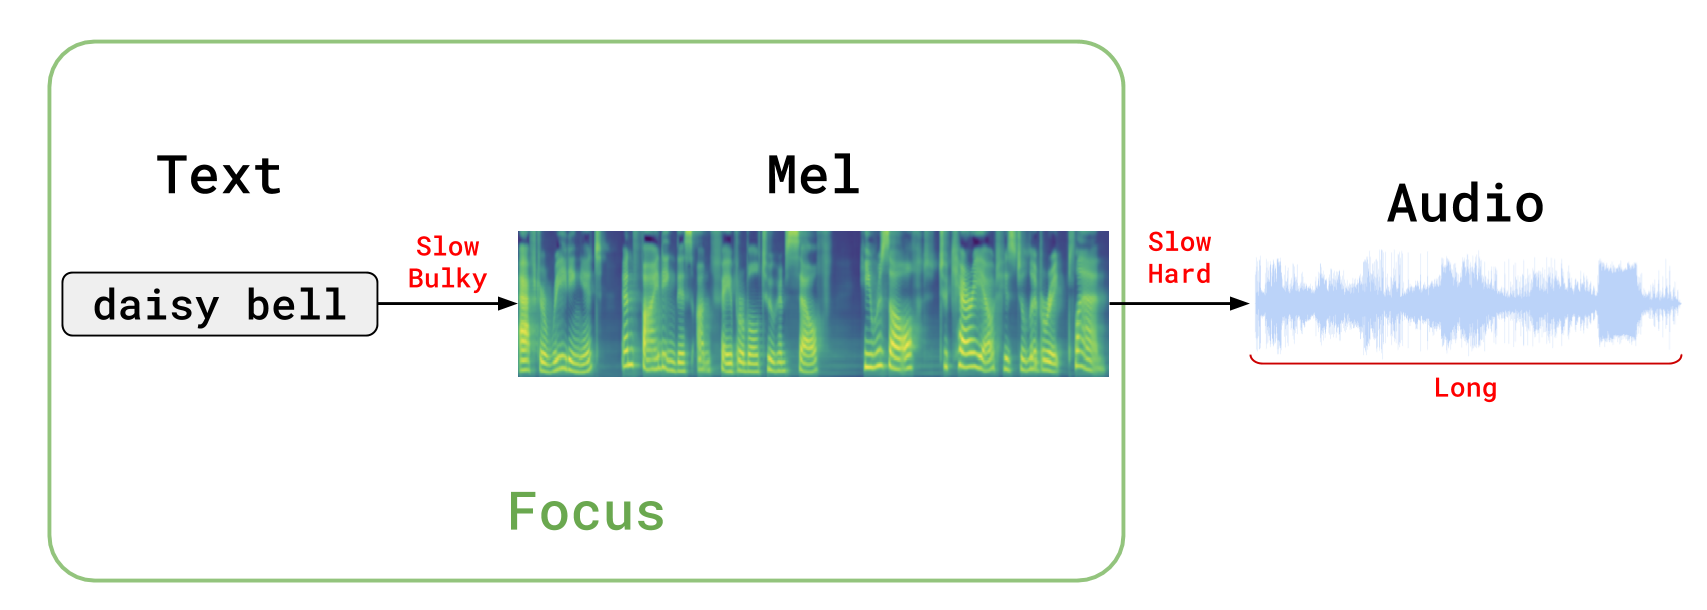
\includegraphics[width=1.0\textwidth]{images/tts-pipeline.png}
\end{figure}
\end{frame}

\begin{frame}
\begin{itemize}
    \item Tacotron2~\footcite{tacotron2}: 30M весов, медленный авторегрессионный вывод (RNN), проблема с устойчивостью
    \item Transformer-TTS~\footcite{transformer-tts}: 60M весов, медленный авторегрессионный вывод, проблема с устойчивостью
    \item FastSpeech~\footcite{fastspeech}: 30M весов, проблемы с обобщением на другие языки, использует Tacotron2 для извлечения данных для обучения (teacher model), механизм внимания
\end{itemize}
\end{frame}

\begin{frame}{Неавторегрессионность}
\begin{figure}[H]
\centering
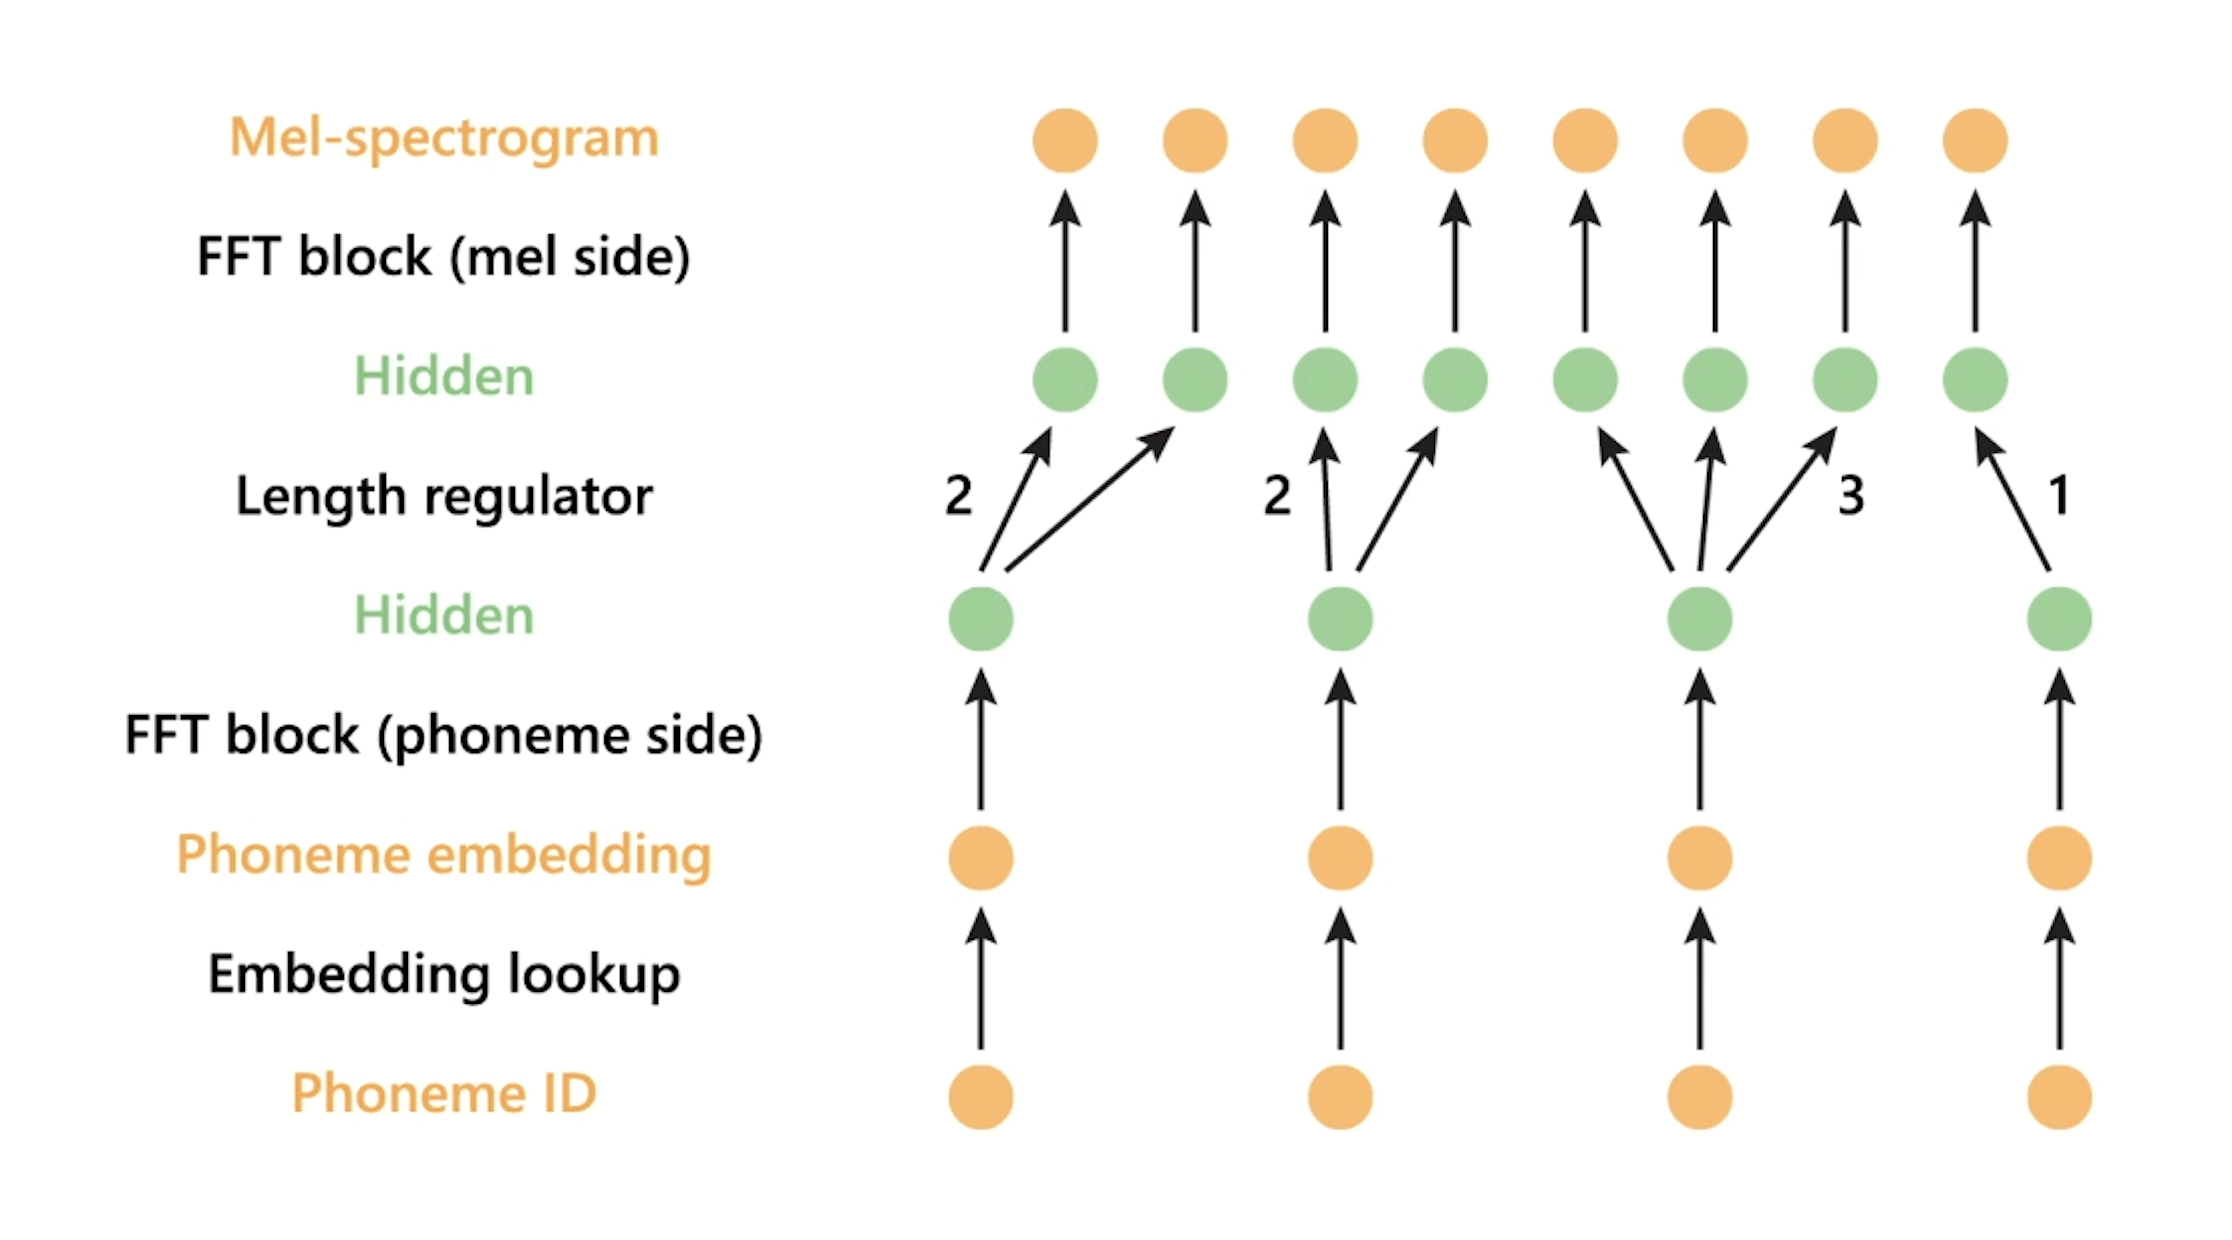
\includegraphics[width=1.0\textwidth]{images/fastspeech/alignment.png}
\end{figure}
\end{frame}

\begin{frame}
\underline{Целью} данной работы является разработка \textbf{легковесной} модели для задачи синтеза речи, позволяющей производить \textbf{быструю, качественную и устойчивую} генерацию. Решение будет основываться на идее неавторегрессионности и конволюционных моделях.

\underline{Задачи}:
\begin{itemize}
    \item Проанализировать предметную область и существующие модели. Обозначить основные проблемы и пути к их решению.
    \item Разработать и описать эффективную архитектуру, основанную на идеи неавторегрессионности.
    \item Выбрать данные для обучения и провести эксперименты.
    \item Произвести сравнение подходов и анализ результатов на качество и скорость.
\end{itemize}
\end{frame}

\section{Архитектура}

\begin{frame}{Идея}
\begin{itemize}
    \item Разделить генерацию на два парралельных этапа: предсказывание длительности графемы и генерация мэл-спектрограммы. Предсказание длительности каждой графемы выравнивает входной текст на мэл по длинне.
    \item Длительности для обучения предсказателя - взять из задачи разпознавания речи (ASR) вместо генерации речи (TTS). В качестве teacher model используется QuartzNet~\footcite{quartznet}.
    \item Введение дополнительного символа ($\sim$), обозначающего промежуточное состояние между соседними символами
    \item Конволюционная неавторегрессионная архитектура
\end{itemize}
\end{frame}

\begin{frame}
\begin{figure}[H]
\centering
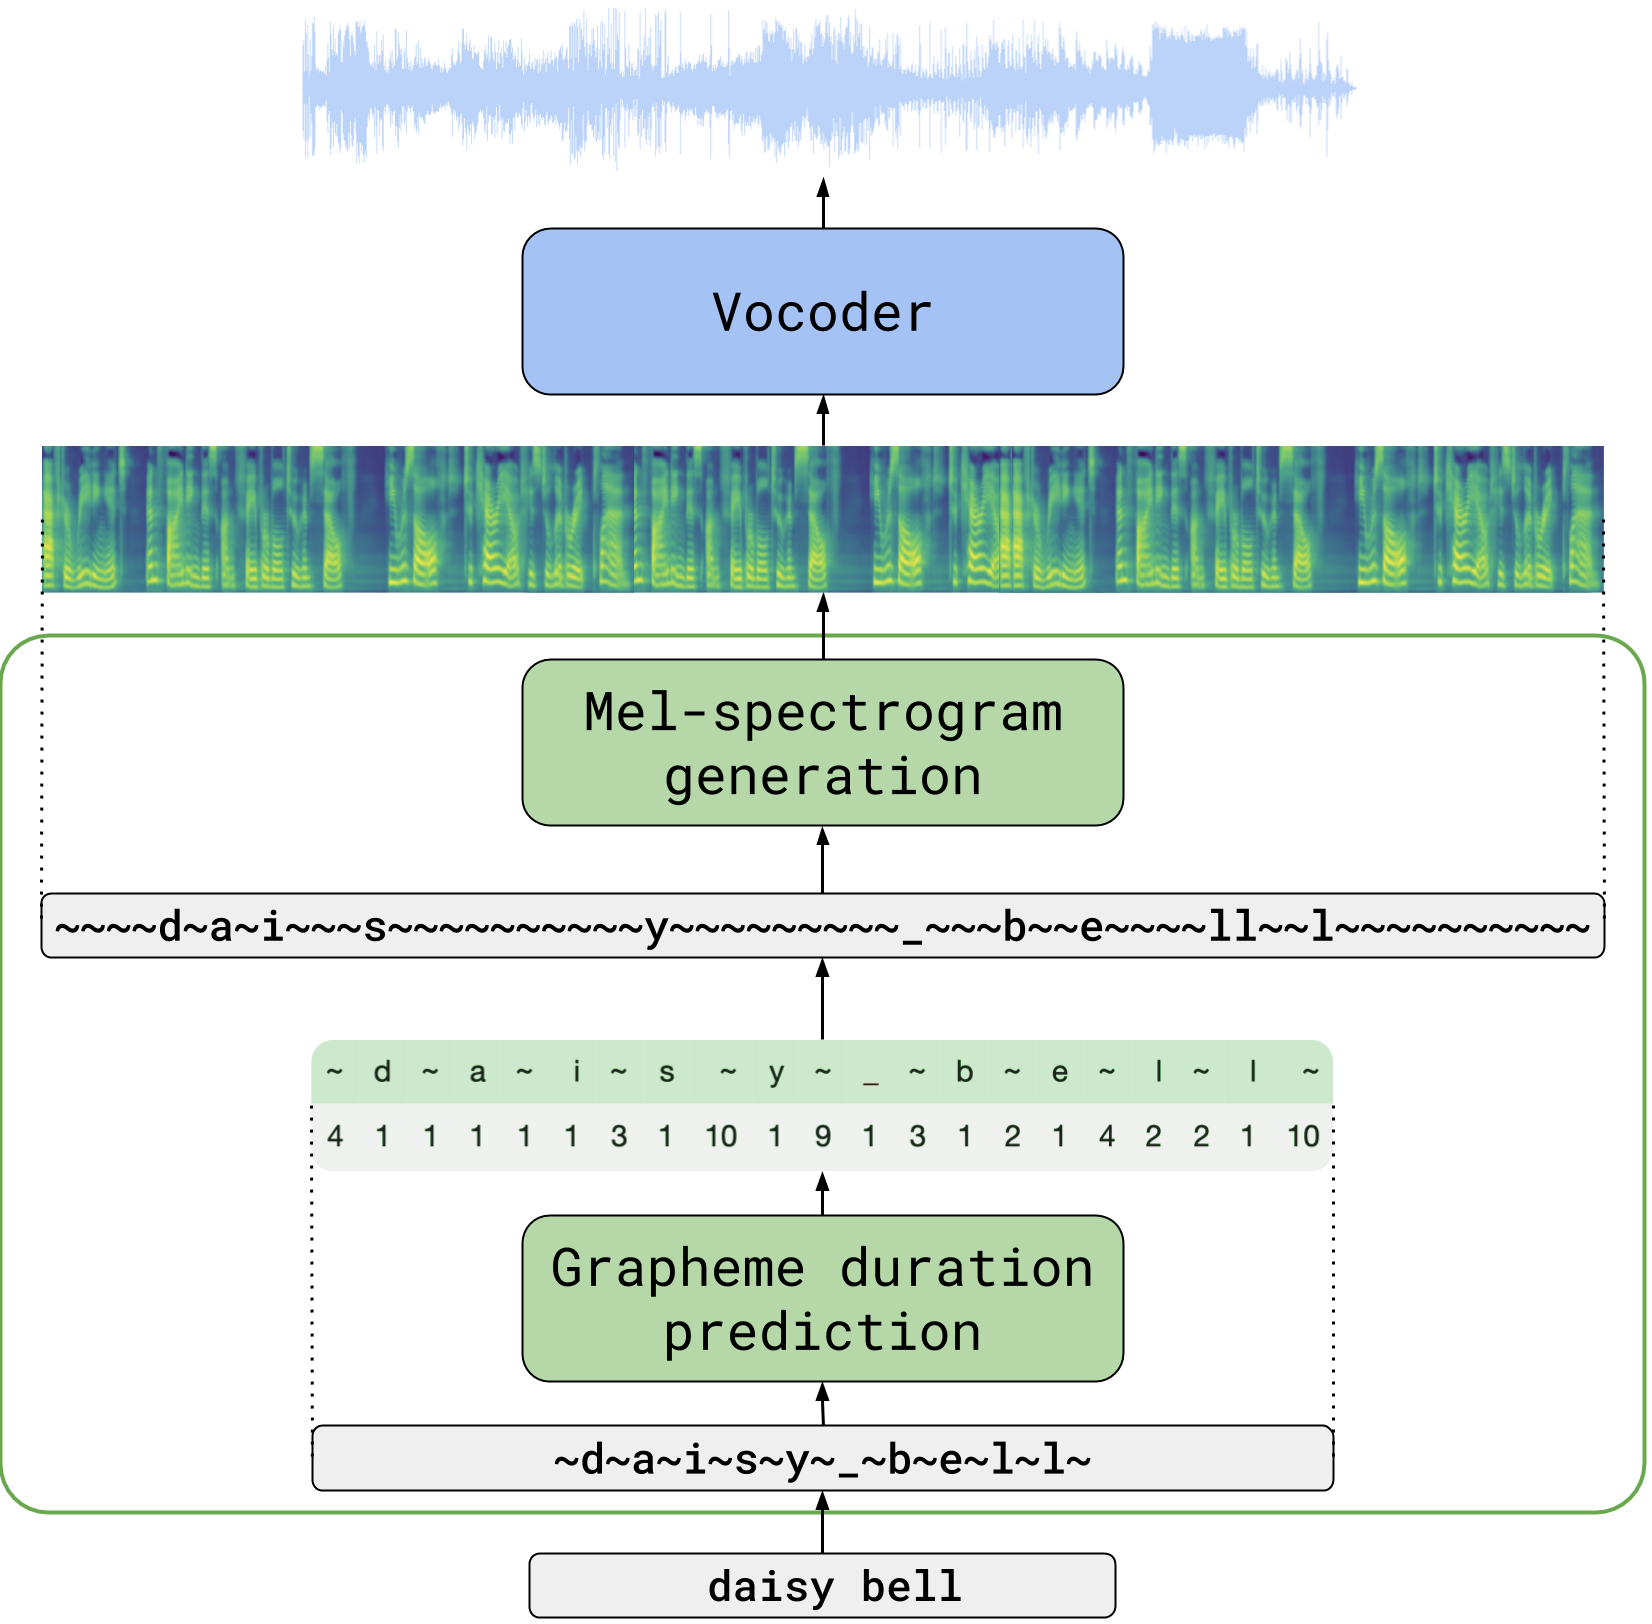
\includegraphics[width=0.7\textwidth]{images/arch.png}
\end{figure}
\end{frame}

\begin{frame}
\begin{figure}[H]
\centering
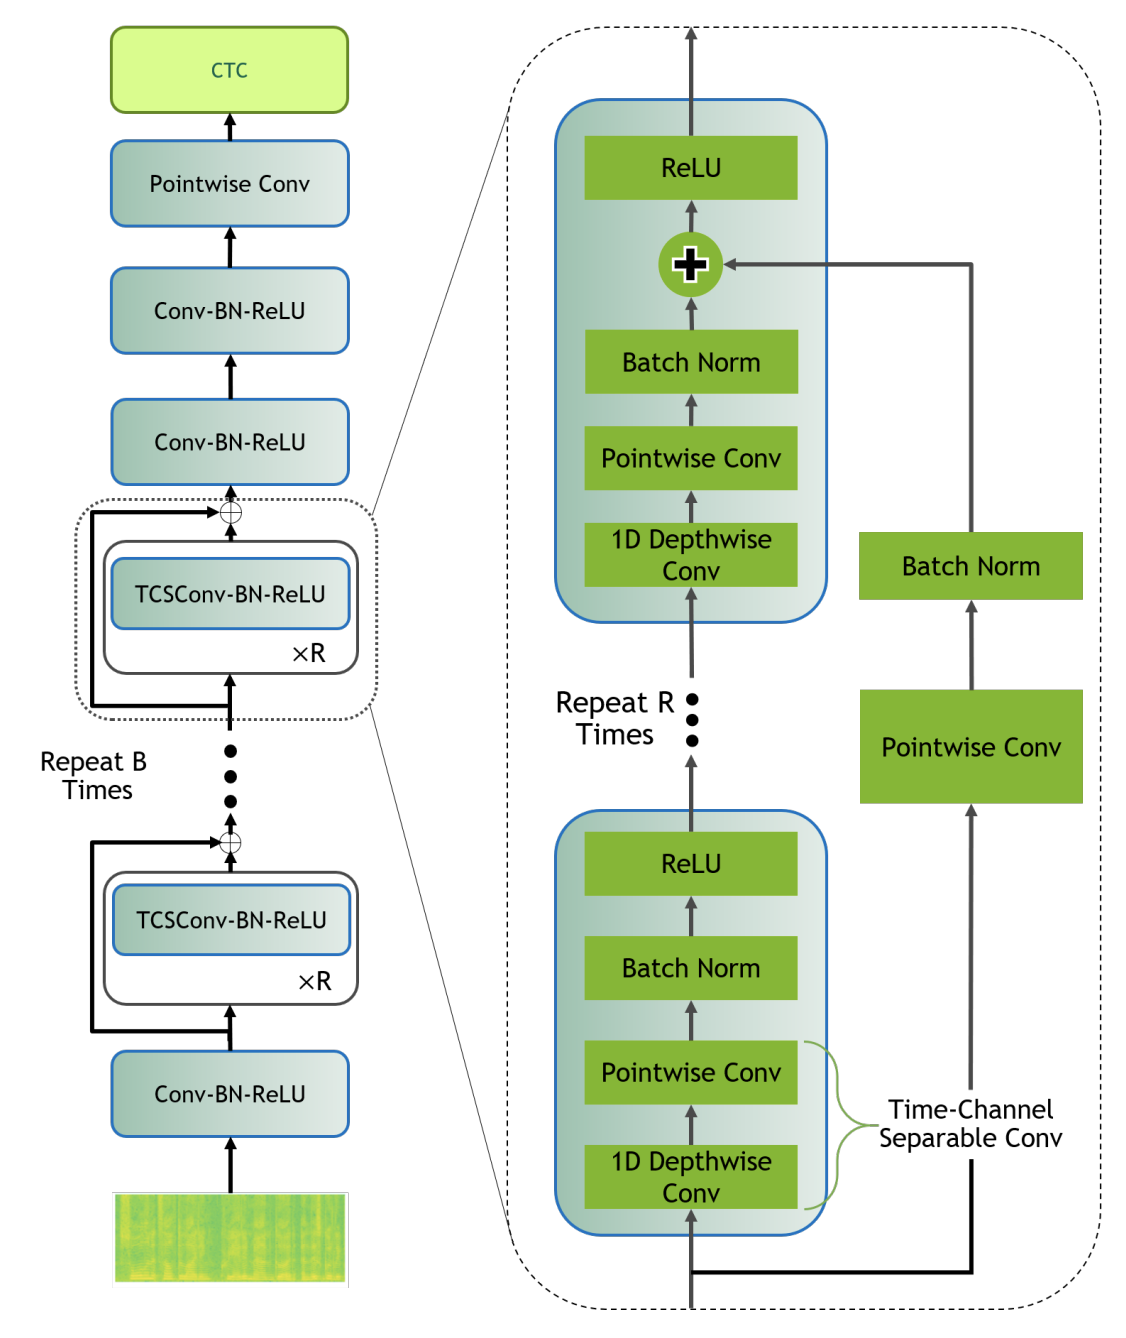
\includegraphics[width=0.5\textwidth]{images/qn.png}
\caption{QuartzNet~\footcite{quartznet} решает обратную задачу: разпознования речи по входному мэлу. Функция ошибки учит выравнивание, из которого извлекаются длительности букв.}
\end{figure}
\end{frame}

\begin{frame}
\begin{figure}[H]
\centering
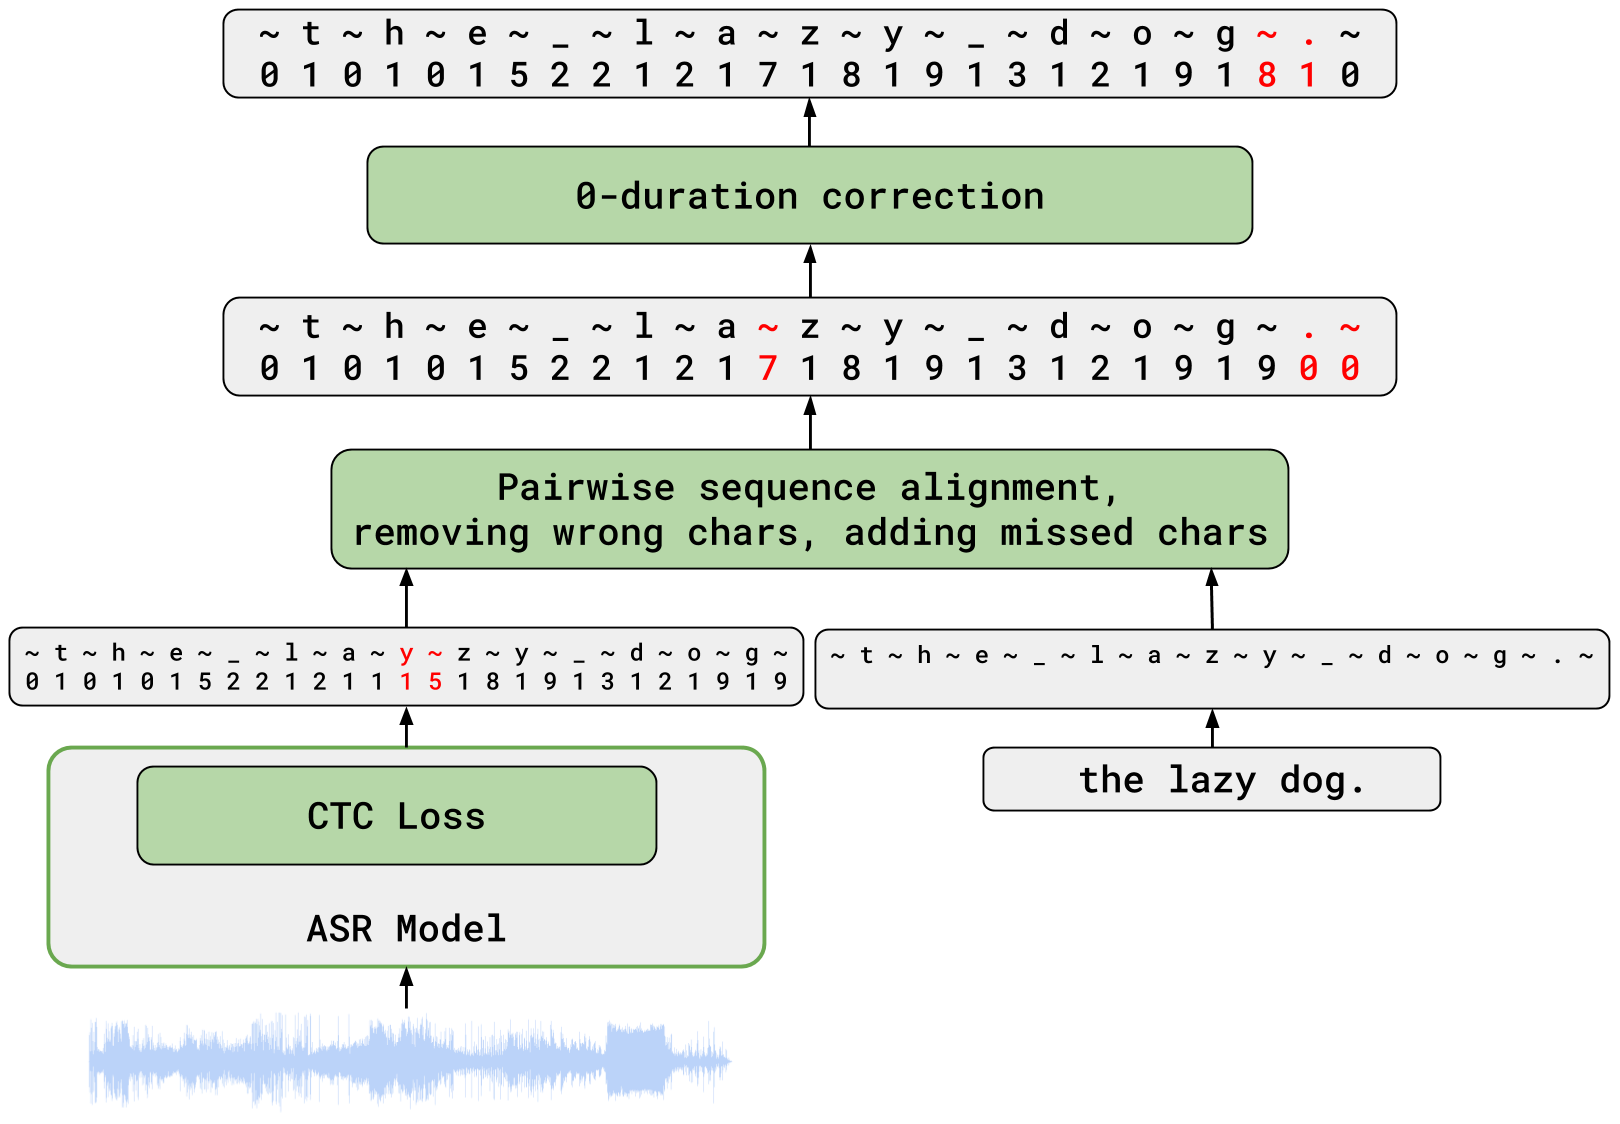
\includegraphics[width=1.0\textwidth]{images/alignment.png}
\end{figure}
\end{frame}

\begin{frame}
\begin{table}[!ht]
\centering
\scalebox{1.0}{
\begin{tabular}{c c c c c} 
\toprule
\textbf{Block} &
\textbf{\thead{\# Sub\\Blocks}} &
\textbf{\thead{\# Output\\Channels}} &
\textbf{Kernel Size} &
\textbf{Dropout} \\
\midrule
Embed & 1 & 256 & 1 & 0.0 \\
Conv1 & 3 & 256 & 3 & 0.0 \\
$B_1$ & 5 & 256 & 5 & 0.0 \\
$B_2$ & 5 & 256 & 7 & 0.0 \\
$B_3$ & 5 & 256 & 9 & 0.0 \\
$B_4$ & 5 & 256 & 13 & 0.0 \\
$B_5$ & 5 & 256 & 15 & 0.0 \\
$B_6$ & 5 & 256 & 17 & 0.0 \\
$B_7$ & 5 & 512 & 21 & 0.0 \\
$B_8$ & 5 & 512 & 23 & 0.0 \\
$B_9$ & 5 & 512 & 25 & 0.0 \\
Conv2 & 1 & 1024 & 1 & 0.0 \\
Conv3 & 1 & 80 & 1 & 0.0 \\
\midrule
\textbf{Params, M} & & & & \textbf{8.5} \\
\bottomrule
\end{tabular}
}
\caption{Mel-spectrogram generator is based on QuartzNet~9x5.}
\end{table}
\end{frame}

\section{Результаты}

\begin{frame}
\begin{table}[!ht]
\centering
\scalebox{1.0}{
\begin{tabular}{l c} 
\toprule
\textbf{Model} &
\textbf{MOS} \\
\midrule
Ground truth speech & $4.31 \pm 0.05$ \\
Ground truth mel + WaveGlow & $4.04 \pm 0.05$ \\
Tacotron 2 + WaveGlow & $3.85 \pm 0.06$ \\
% FastSpeech~\cite{Fastspeech2019} & $\star \pm \star$ \\
\midrule
TalkNet + WaveGlow & $3.74 \pm 0.07$ \\
\bottomrule
\end{tabular}
}
\caption{MOS scores with $95\%$ confidence interval}
\end{table}
\end{frame}

\begin{frame}
\begin{table}[!ht]
\centering
\scalebox{1.0}{
\begin{tabular}{l l l r} 
\toprule
\textbf{Model} & 
\textbf{Batch} &
\textbf{Latency, s} &
\textbf{RTF} \\
\midrule
Transformer TTS & 1 & $6.735 \pm 3.969$ & $1.48 \pm 0.87$ \\
Tacotron 2 & 1 & $0.817 \pm 1\cdot 10^{-2} $ & $7.56 \pm 0.01$ \\
FastSpeech & 1 & $0.029 \pm 2 \cdot {10}^{-4}$ & $221.01 \pm 1.75$ \\
\midrule
TalkNet & 1 & $0.019 \pm 1 \cdot {10}^{-5}$ & $328.65 \pm 4.76$ \\
TalkNet & 4 & $0.023 \pm 5 \cdot {10}^{-5}$ & $1048.80 \pm 21.75$ \\
TalkNet & 8 & $0.037 \pm 4 \cdot {10}^{-4}$ & $1340.09 \pm 8.90$ \\
\bottomrule
\end{tabular}
}
\caption{TalkNet inference latency for mel-spectrogram generation (without vocoder). The latency was measured with batch size $1$ using a V100 GPU and averaged over 2048 samples from LJSpeech. Latency and Real-Time-Factor (RTF) with $95\%$ confidence interval.}
\end{table}
\end{frame}

\begin{frame}
\begin{figure}[H]
\centering
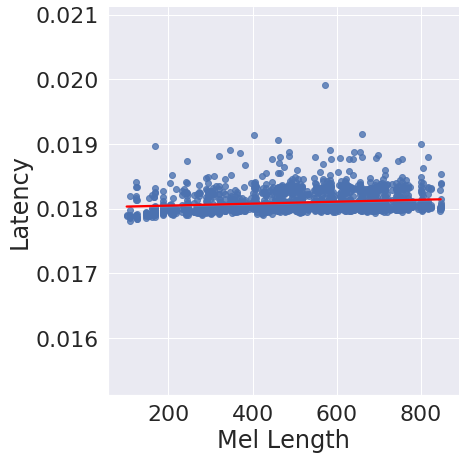
\includegraphics[width=0.6\textwidth]{images/len-lat.png}
\caption{Эффект неавторегрессионности и отсутствия механизма влияния (attention).}
\end{figure}
\end{frame}

\begin{frame}{Результаты}
\begin{itemize}
    \item $300$x realtime генерация
    \item 10M весов: уменьшение в 3 раза
    \item Новая 2ух шаговая архитектура
    \item ASR в качестве учителя вместо TTS
    \item Отсутствует механизм внимания (attention)
    \item Статья~\footcite{beliaev2020talknet}
\end{itemize}
\end{frame}

\begin{frame}{Литература}
\printbibliography[heading=none]
\end{frame}

\end{document}